\begin{center}
    \begin{figure}[H]
        \centering

        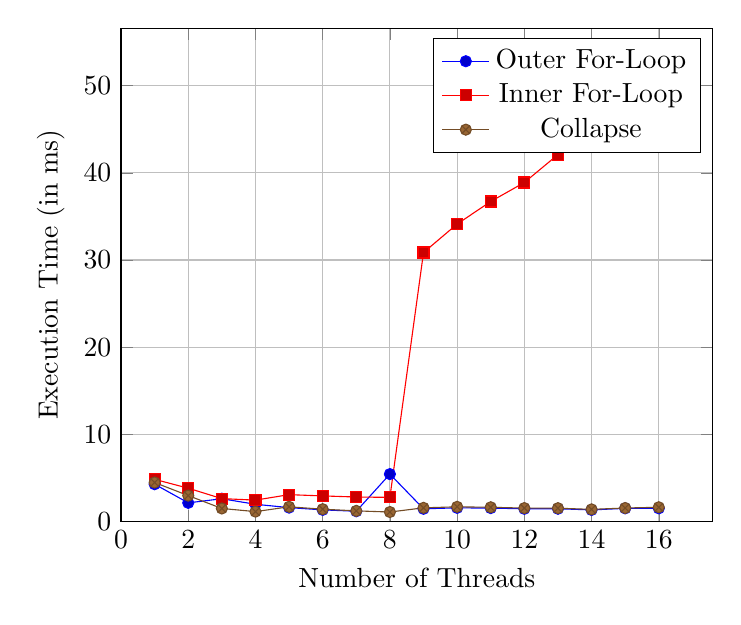
\begin{tikzpicture}
            \begin{axis}[
                title={},
                width=0.75\textwidth,
                xlabel={Number of Threads},
                ylabel={Execution Time (in ms)},
                xmin=0,
                ymin=0,
                grid=major
            ]
                \addplot coordinates {
                    (1,4.25925)(2,2.11895)(3,2.5918)(4,1.9537)(5,1.572)(6,1.31315)(7,1.15475)(8,5.41915)(9,1.43565)(10,1.5453)(11,1.5184)(12,1.4348)(13,1.44295)(14,1.30675)(15,1.48805)(16,1.48985)
                };
                \addlegendentry{Outer For-Loop}

                \addplot coordinates {
                    (1,4.8171)(2,3.7998)(3,2.60445)(4,2.43305)(5,3.0599)(6,2.9158)(7,2.7888)(8,2.74855)(9,30.8562)(10,34.1217)(11,36.713)(12,38.8938)(13,42.0953)(14,49.7418)(15,48.6)(16,51.4584)
                };
                \addlegendentry{Inner For-Loop}       

                \addplot coordinates {
                    (1,4.4527)(2,2.95205)(3,1.47325)(4,1.11305)(5,1.66655)(6,1.3907)(7,1.1971)(8,1.06665)(9,1.5488)(10,1.66275)(11,1.61175)(12,1.5165)(13,1.5057)(14,1.3701)(15,1.5257)(16,1.6131)
                };
                \addlegendentry{Collapse}
            \end{axis}
        \end{tikzpicture}
        \caption{Grayscale Performance Tests pnglogo-blk.png}
    \end{figure}
\end{center}